\section{Algorithm} % (fold)

Before taking deep look into the methods, input and output need to be defined. The input is pedestal subtracted PMT waveform (see figure~\ref{fig:input}), and the output is the charge or penumber sequence (see figure~\ref{fig:output}). 

\begin{figure}[H]
\begin{minipage}{.5\textwidth}
\begin{figure}[H]
    \centering
        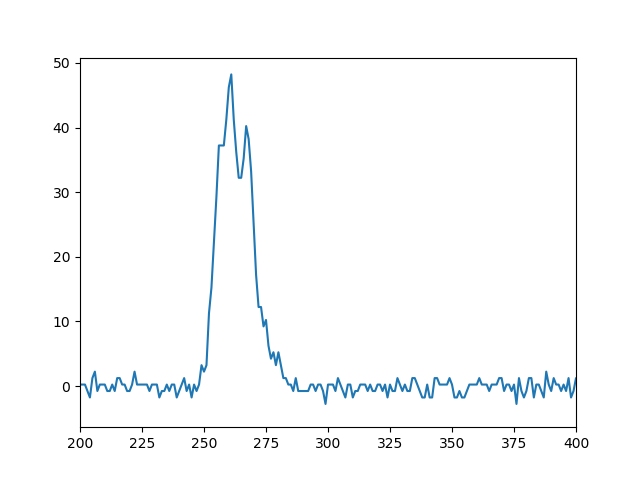
\includegraphics[width=1.0\textwidth]{figures/wave.png}
    \caption{\label{fig:input} Data input}
\end{figure}
\end{minipage}
\begin{minipage}{.5\textwidth}
\begin{figure}[H]
    \centering
        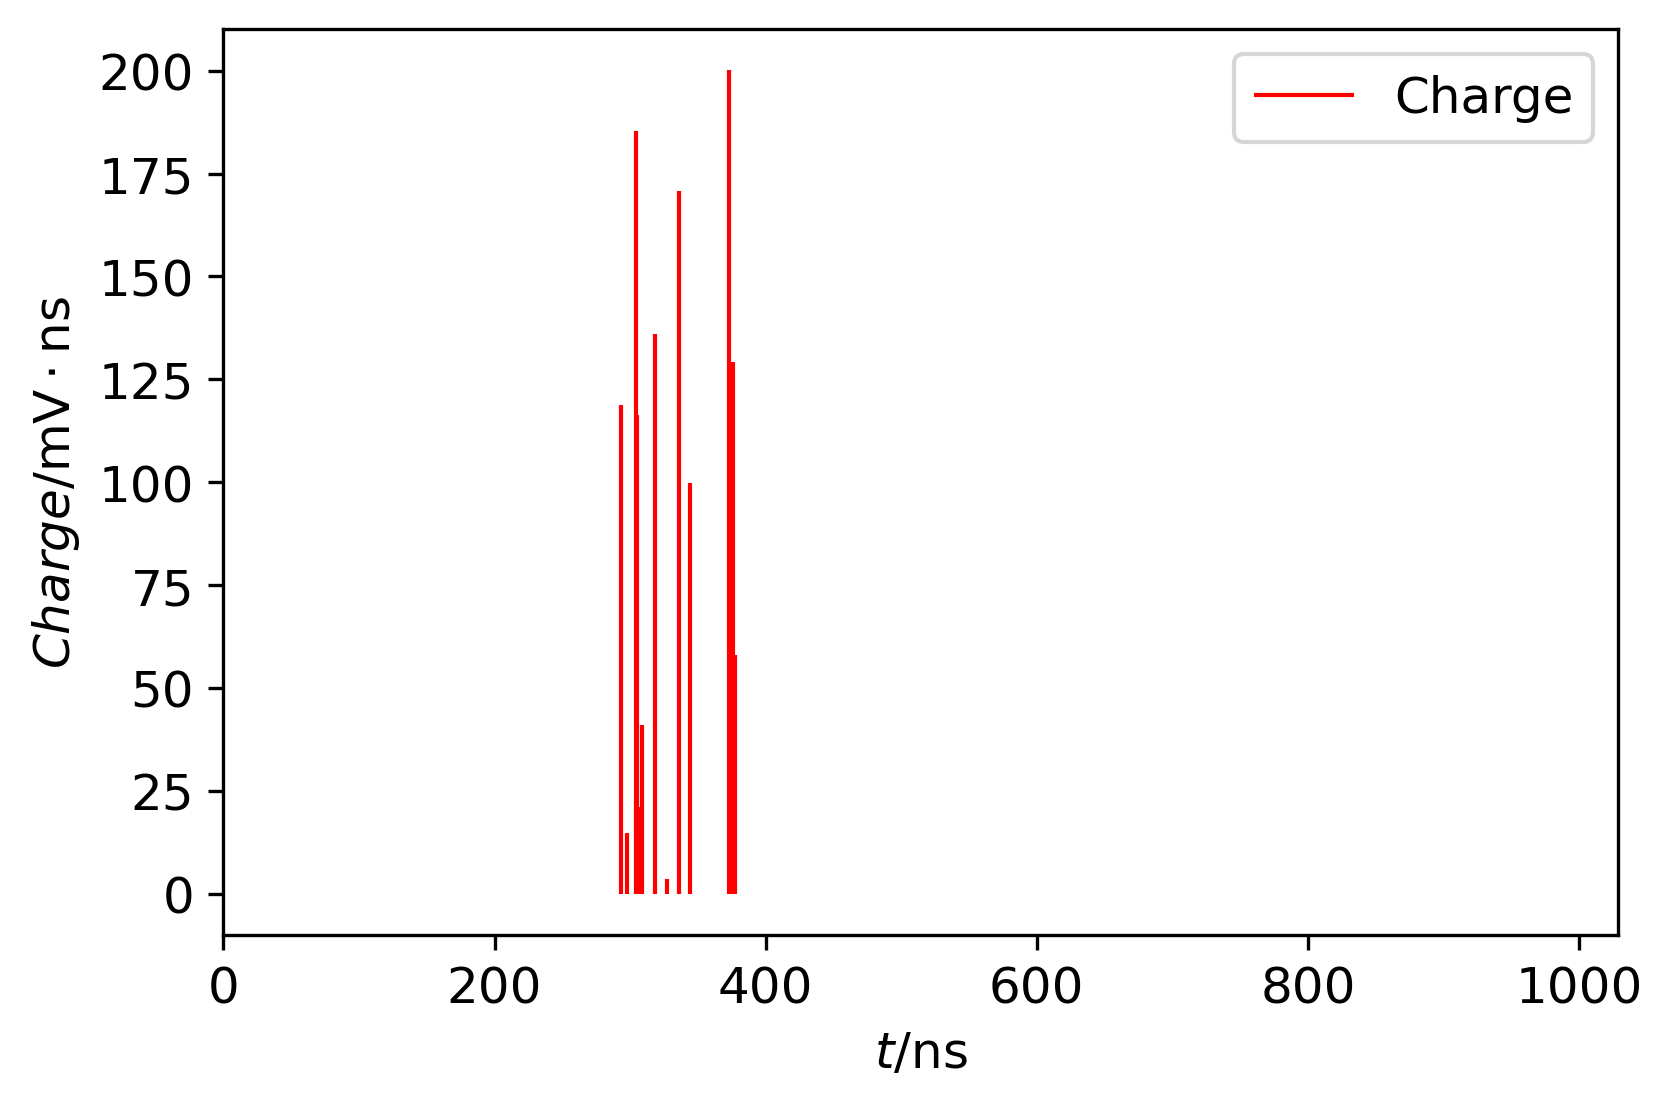
\includegraphics[width=1.0\textwidth]{figures/charge.png}
    \caption{\label{fig:output} Data output}
\end{figure}
\end{minipage}
\end{figure}

Total photo-electron number is the count of hittime. The histogram of Total photo-electron number and data structure show in figure (see figure~\ref{fig:penum}). 

\begin{figure}[H]
\begin{minipage}{.5\textwidth}
\begin{figure}[H]
    \centering
        \includegraphics[width=1.0\textwidth]{figures/penum.png}
    \caption{\label{fig:penum} TotalPEnum Histogram}
\end{figure}
\end{minipage}
\begin{minipage}{.5\textwidth}
\begin{figure}[H]
    \centering
        \includegraphics[width=0.7\textwidth]{figures/dataset.png}
    \caption{\label{fig:set} Data Structure}
\end{figure}
\end{minipage}
\end{figure}

\subsection{Find peak}
First intuitive method is find peak method. First we find the peak of waveform, then we move leftward. The delta t we move is the peak time of single pe response. 

\begin{figure}[H]
    \centering
    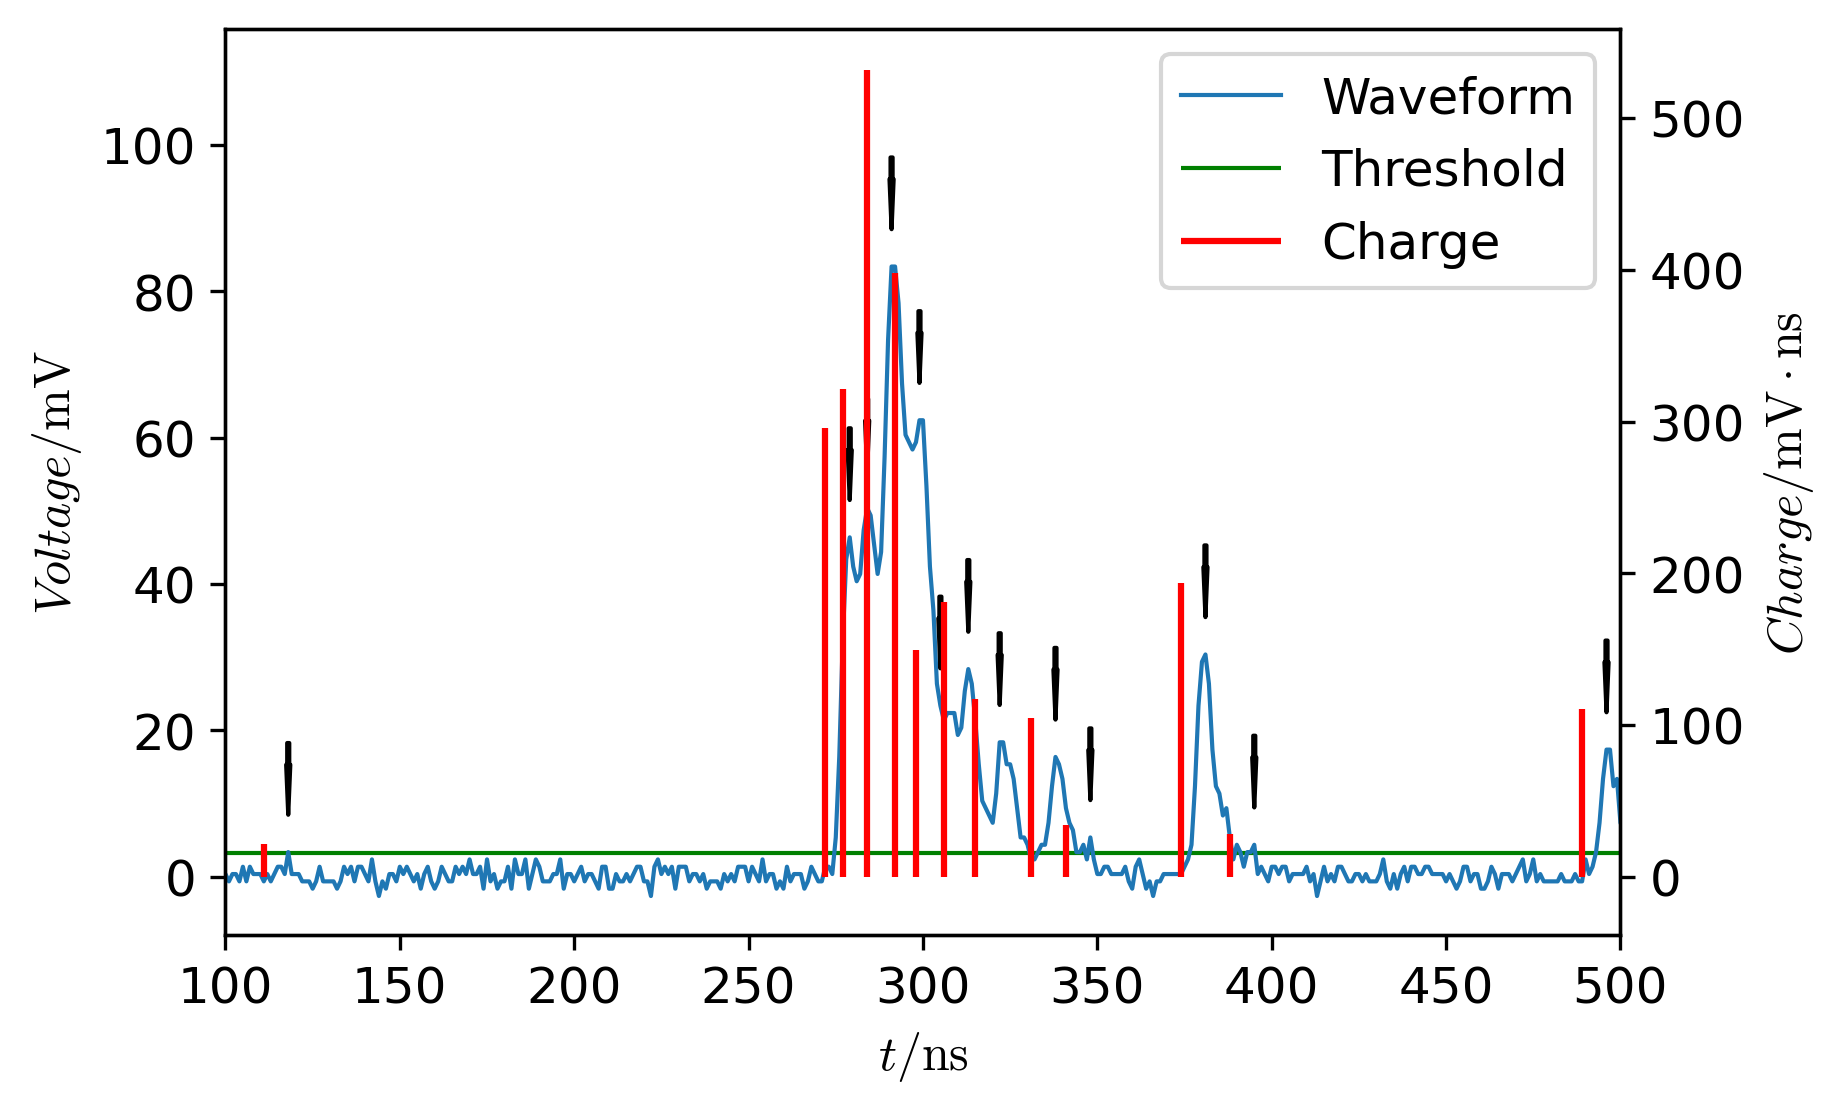
\includegraphics[width=0.6\linewidth]{figures/findpeak.png}
    \caption{Find Peak Method Demo, W-dist = 4.02}
\end{figure}

\subsection{Waveform shift}
A threshold is settled with respect to noise in simulation data. In waveform shift method, first we locate the part of waveform exceeds threshold. Then we shift the exceeding part leftward. The time length shifted is referenced to single PE response. And treat the normalized exceeding part as charge or penum. 

\begin{figure}[H]
    \centering
    \includegraphics[width=0.6\linewidth]{figures/threshold.png}
    \caption{Waveform Shift Method Demo, W-dist = 10.75}
\end{figure}

\subsection{Fourier transform deconvolution}
Third method is Fourier deconvolution. Assuming that the waveform is the convolution of single pe response and hittime sequence, the fft of waveform and single pe response are computed. A rectangular filter is added. Then compute the inverse fft of the quotient of filtered fft of waveform and fft of single pe response. 

\begin{itemize}
    \item Results = IFFT\{ Filter[ FFT(Waveform) / FFT(SPE) ] \}
\end{itemize}

\begin{figure}[H]
    \centering
    \includegraphics[width=0.6\linewidth]{figures/fftrans.png}
    \caption{Fourier Deconvolution Demo, W-dist = 1.63}
\end{figure}

\subsection{Lucy deconvolution}
Lucy-Richardson deconvolution is a non linear iteration method, to calculate the deconvolution of signals. Lucy deconvolution has an advantage against Fourier deconvolution which is a constraint that charge or penum are larger than 0. 

\begin{figure}[H]
    \centering
    \includegraphics[width=0.6\linewidth]{figures/lucyddm.png}
    \caption{Lucy Deconvolution Demo, W-dist = 1.25}
\end{figure}

\subsection{Fitting}
First we extract enough single PE response from simulation data in fitting method. We suppose the average of these waveforms is the single PE response. In fitting process, the parameter is weight in each discrete hittime. The loss which we need to optimize is the truth wave and reconstructed wave according to the parameters. The graph here shows one of the fitting result. We can see the truth waveform and reconstructed waveform is very similar. 

\begin{figure}
    \centering
    \includegraphics[width=0.5\linewidth]{figures/demo.png}
    \caption{Fitting Demo, W-dist = 2.23}
\end{figure}

\begin{figure}[H]
\begin{minipage}{.5\textwidth}
\begin{figure}[H]
    \centering
        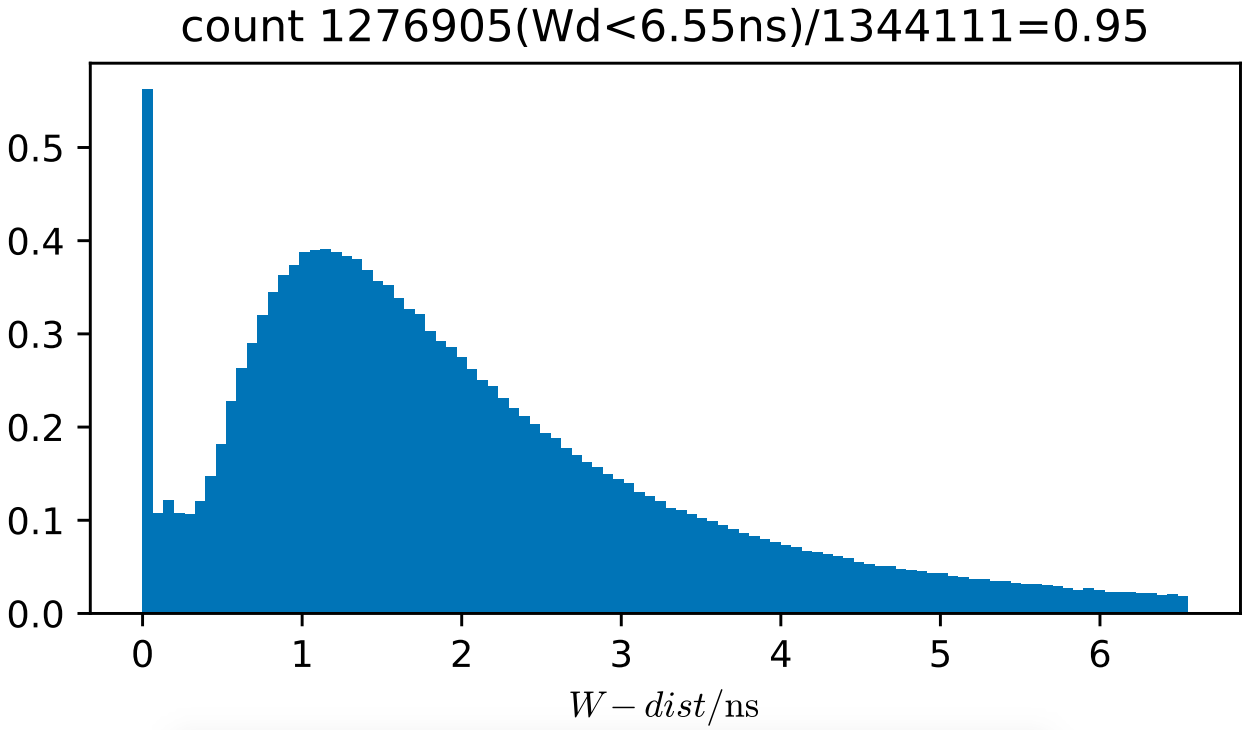
\includegraphics[width=1.0\textwidth]{figures/xiaopeippenumhist.png}
    \caption{Fitting \#PE Result Histogram}
\end{figure}
\end{minipage}
\begin{minipage}{.5\textwidth}
\begin{figure}[H]
    \centering
        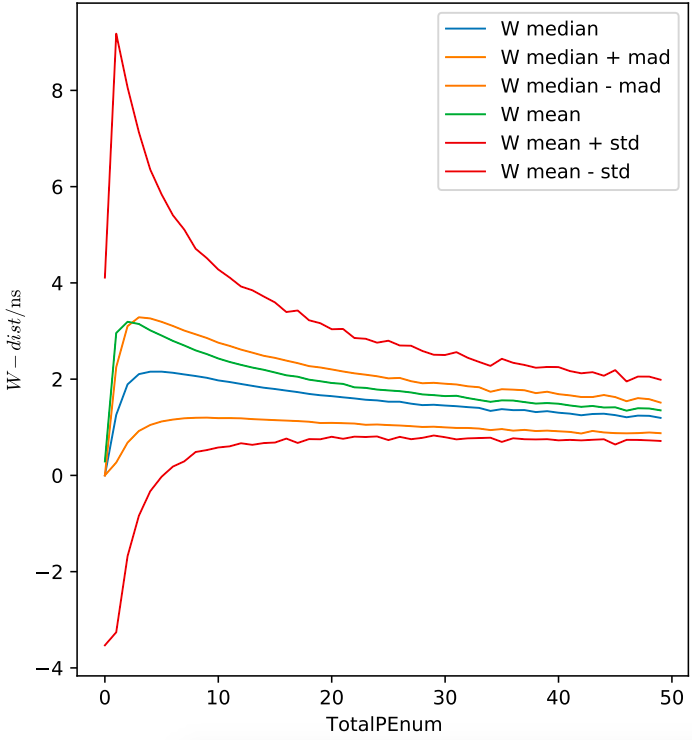
\includegraphics[width=0.7\textwidth]{figures/xiaopeippenumstats.png}
    \caption{Fitting \#PE W-dist vs TotalPEnum}
\end{figure}
\end{minipage}
\end{figure}
\begin{figure}[H]
\begin{minipage}{.5\textwidth}
\begin{figure}[H]
    \centering
        \includegraphics[width=1.0\textwidth]{figures/xiaopeipchargehist.png}
    \caption{Fitting Charge Result Histogram}
\end{figure}
\end{minipage}
\begin{minipage}{.5\textwidth}
\begin{figure}[H]
    \centering
        \includegraphics[width=0.7\textwidth]{figures/xiaopeipchargestats.png}
    \caption{Fitting Charge W-dist vs TotalPEpos}
\end{figure}
\end{minipage}
\end{figure}

% \subsection{CNN}
\subsection{CNN}

\subsubsection{Network structure}
%\subsection{What is a good Network Structure?} 

Advances in neural networks have brought breakthroughs in various domains like Computer Vision and Natural Language Processing. As an efficient composition with weighted additions and pointwise nonlinearities, the method has prevailed against most of the traditional algorithms in pattern recognition tasks. In our experiment, we introduced a multi-layer convolutional neural network to process time-sensitive signals from detector outputs. Based on the Physics nature that a detector signal (PMT outputs) do only have a local correlation with recent incoming particles (photons incidents), we chose convolutional setups with a moderate total width coverage. From a view of information, a broader coverage by an output neuron's receptive field on its related area will contribute to higher accuracy, while redundant connections could only lead to excessive computation and lower processing speed. As a result, a wise setup should try to cover all relevant signal areas exclusively while cutting off every connection unnecessary, balancing the speed and accuracy from the two mentioned effects.

A similar trade-off also exists in the depth of the neural network. A deeper network could provide more complex combinations to all detected features, and the computation complexity of result calculation changes linearly with the depth. With the existence of advanced structure like residual connection and strategies like batch-norm, depth in training is never a problem. However, to cut the computation in massive experimental data, a network should be relatively shallow. Detector signals are relatively similar and peak-shaped. Such a simple pattern does not require many layers to recognize. A good design for the task is a network with 4 to 6 layers. Deeper structures may bring a slight improvement in precision but will introduce a considerable increase in processing cost.

A convolutional neural network is developed to analys the waveform. Here is the structure of CNN which has 5 convolutional layer (see figure~\ref{fig:struct}). The length of data remains the same. 

\subsubsection{Processing workflow}
%\subsection{What is a complete workflow of Data Processing?}
The complete workflow of data processing consists of two stages, data training and predicting. Data training is a task of supervised learning.  Based on paired data examples, the goal is to find an efficient mapping from detector waves to particle incidents with backpropagation methods. In the training process, a loss function judges the difference between training outputs and their referenced truth, and the training process is to minimize the loss. The product of network training is a function that creates desired outputs from inputs. By directly putting waveforms as inputs, one can get demanded outputs from a trained network in prediction.
%<Add a workflow description here>

\subsubsection{Loss function}
%\subsection{What is a good Loss Function?}
A critical issue matters the network training is the loss function. Particle incidence only happens in a small proportion of time channels within a recorded sequence, which means the outputs and related truth are always sparse. While operating with ineffective loss functions, training processes always ends up in local optimal of constant output due to the sparsity. Also, in practice, the form of loss function influence heavily on the final prediction performance. 

A well-designed loss function should meet two requirements as follows: it should handle the sparsity, and it should give a fair judgement to the output in training. A qualified loss function could work on either sequence values or normalized distributions. In pursuit of time precision, a good algorithm should encourage correct predictions in the close neighbourhoods of their corresponding truth, while punishing outputs that are incorrect or inaccurate in time. While working on the sequence outputs, such a mechanism is easy to implement but hard to arrange appropriately. It is hard to find a fair arrangement of punishment weight matching all circumstance. On the other hand, statistical distances and divergences could assess the difference in distribution but are hard to implement in a trainable form for backpropagation. 

To tackle the mentioned difficulties, efforts of our work have established feasible, robust solutions with guaranteed performance and convergence for each case of processing. We will describe the details of the method in the following section.

\emph{Value-based Reconstruction Loss}
% Introductory Photos should be added to this part.
To cope with sparsity in value-based processing, we have introduced a reconstruction procedure to build up a waveform based on its corresponding particle incidences. By introducing a reverse process after neural network computing, one could define the loss function on a denser wave domain instead of the original incidence domain. Expression of the reconstruction is arbitrary but should fit the paired relationship expressed by data samples. Typically, one should add a training process to fit the parameters in construction expressions before training the predicting neural networks.
%<Add an algorithm description here>

\emph{CDF Wasserstein Loss}
A direct implementation of judgement metrics into loss function is often difficult. To deal with sparsity and encourage time accuracy, we established the loss function on the cumulative distribution functions (CDF) of normalized outputs. The form of cumulative sums could build a connection between sequence prediction and its previous values, making optimization through history possible. Moreover, the first Wasserstein distance between two 1D distributions is equivalent to the norm-1 difference of two corresponding CDFs. The optimal transport amount described by this metric is a reliable measurement standard to all distribution differences, including cases in our application.

\begin{figure}[H]
\begin{minipage}{.3\textwidth}
\begin{figure}[H]
    \centering
    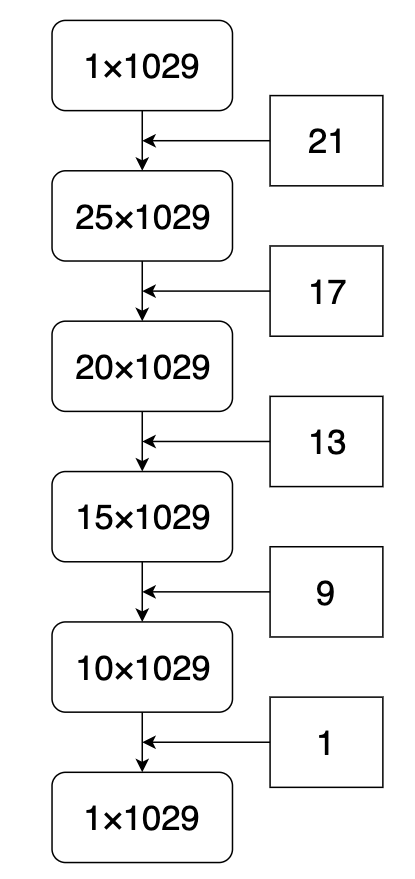
\includegraphics[width=0.8\textwidth]{figures/model.png}
    \caption{\label{fig:struct} CNN Structure}
\end{figure}
\end{minipage}
\hspace{4mm}
\begin{minipage}{.7\textwidth}
\lstinputlisting[language=Python, basicstyle=\small]{figures/CNN}
\end{minipage}
\end{figure}

In the training process, we trained CNN for each PMT channel. The loss which is Wasserstein distance during training show in figure \ref{fig:loss}. 

\begin{figure}[H]
    \centering
    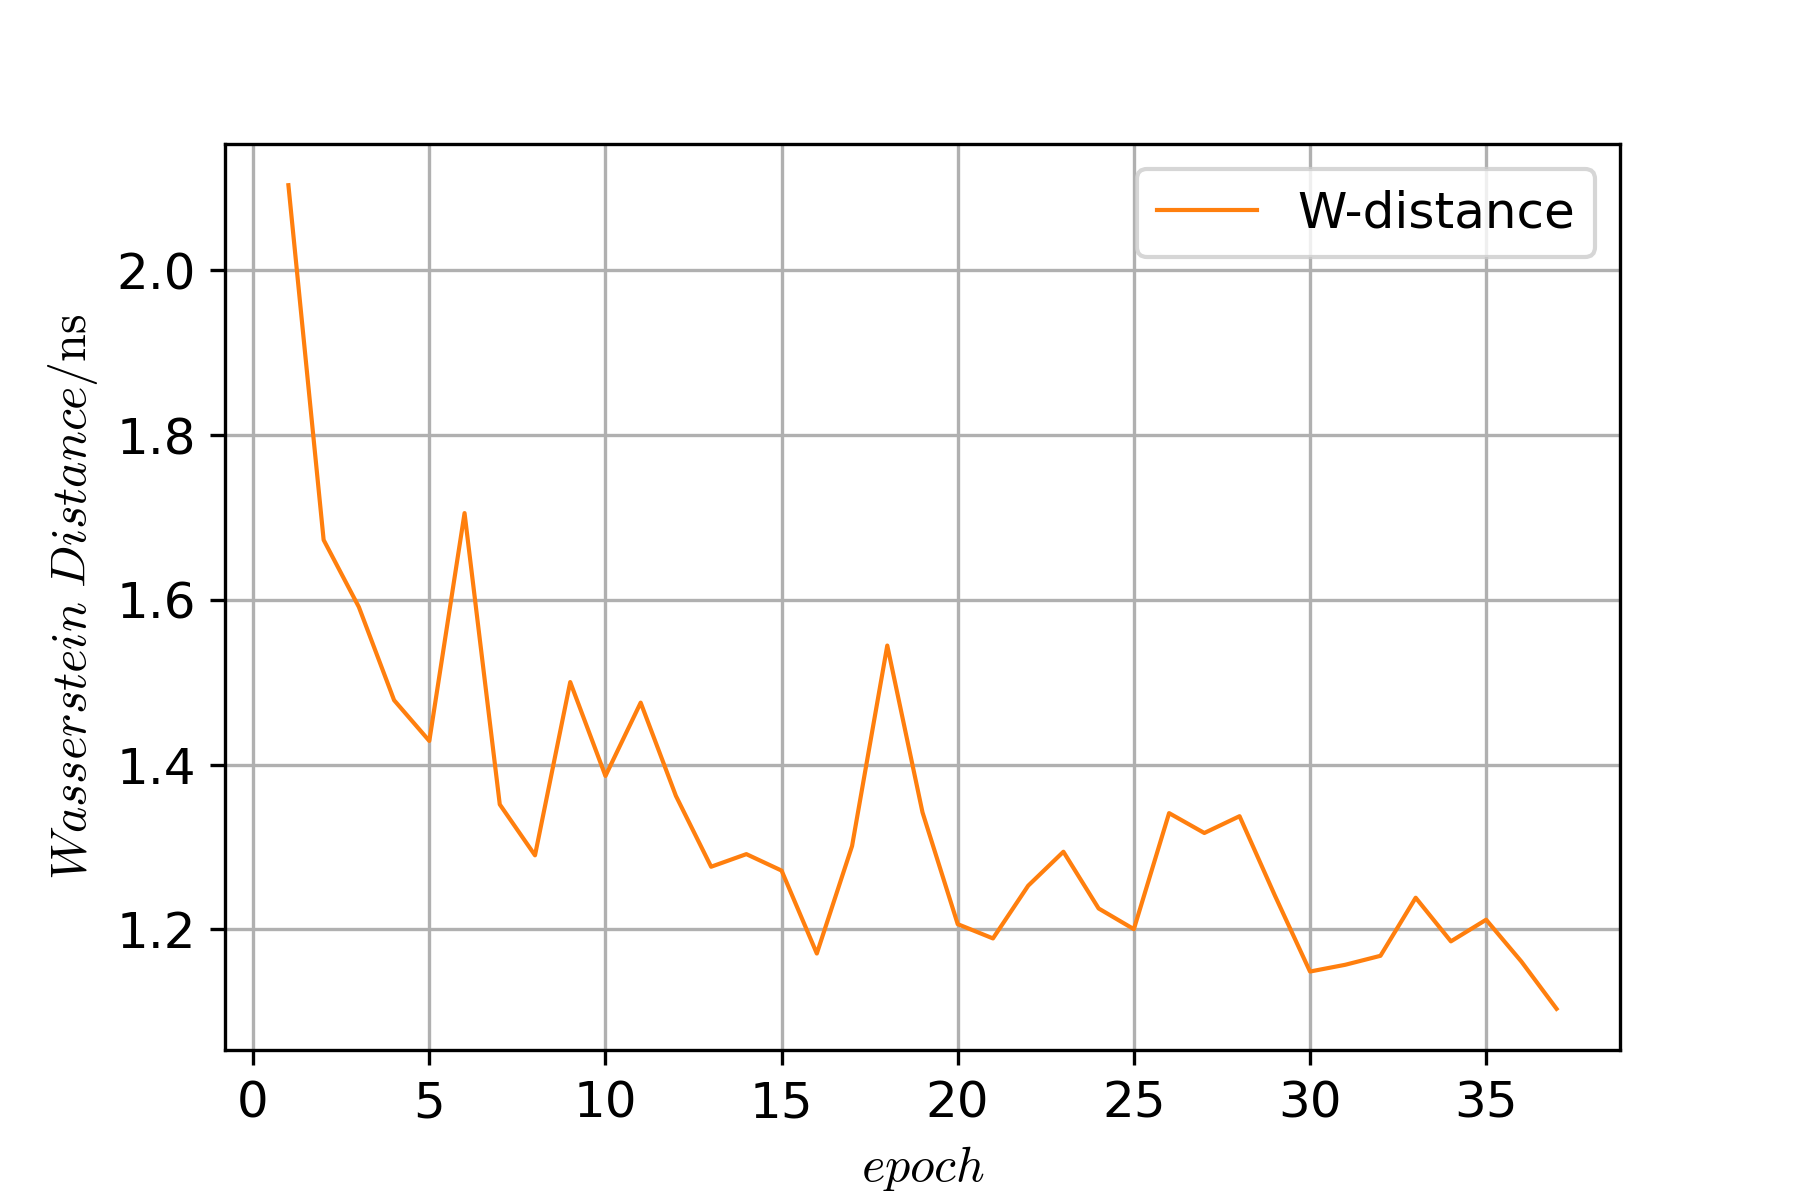
\includegraphics[width=0.6\linewidth]{figures/epoch.png}
    \caption{\label{fig:loss} Loss variation during training}
\end{figure}

The result shows that CNN is the best for reconstruction of Charge and \#PE. 

\begin{figure}[H]
\begin{minipage}{.5\textwidth}
\begin{figure}[H]
    \centering
        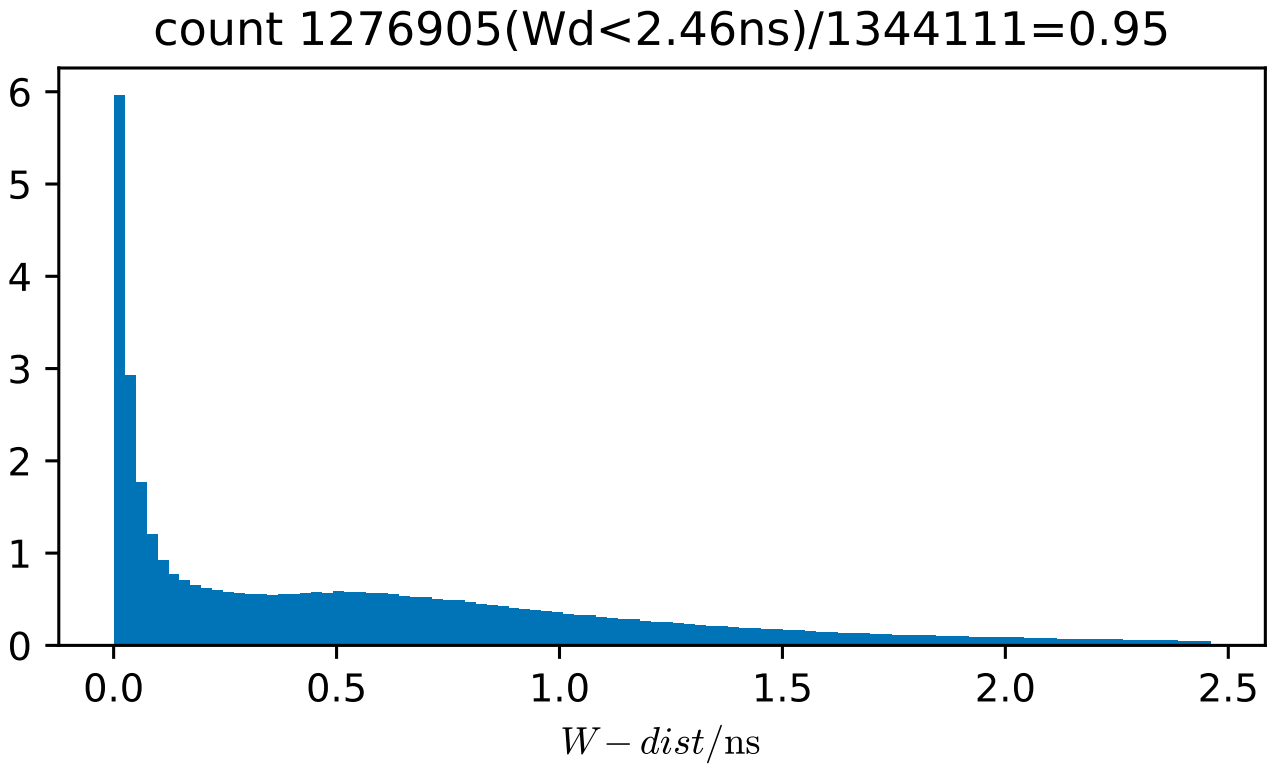
\includegraphics[width=1.0\textwidth]{figures/takarapenumhist.png}
    \caption{CNN \#PE Result Histogram}
\end{figure}
\end{minipage}
\begin{minipage}{.5\textwidth}
\begin{figure}[H]
    \centering
        \includegraphics[width=0.7\textwidth]{figures/takarapenumstats.png}
    \caption{CNN \#PE W-dist vs TotalPEnum}
\end{figure}
\end{minipage}
\end{figure}
\begin{figure}[H]
\begin{minipage}{.5\textwidth}
\begin{figure}[H]
    \centering
        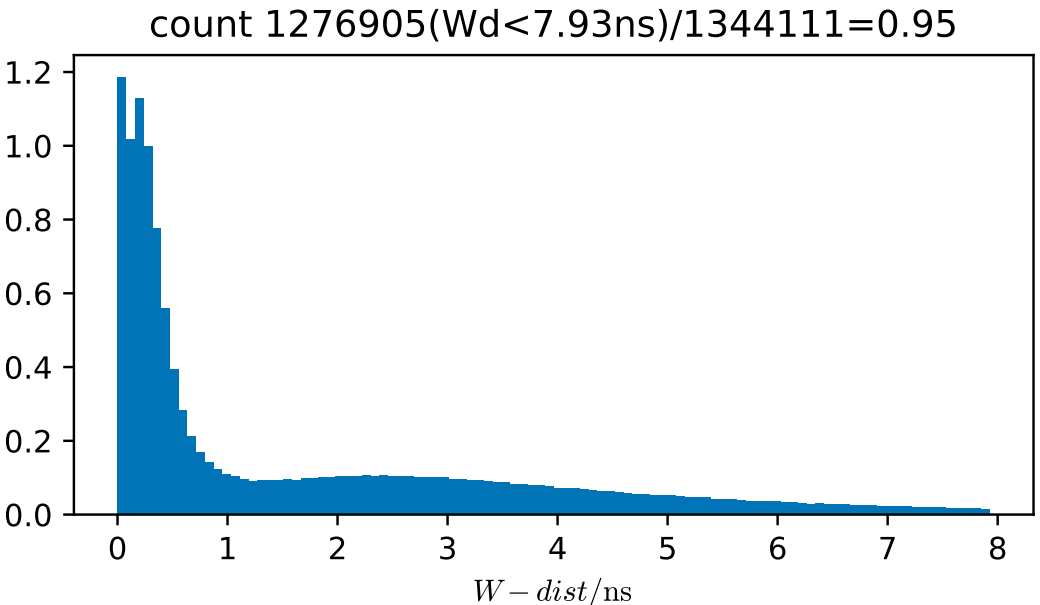
\includegraphics[width=1.0\textwidth]{figures/takarachargehist.png}
    \caption{CNN Charge Result Histogram}
\end{figure}
\end{minipage}
\begin{minipage}{.5\textwidth}
\begin{figure}[H]
    \centering
        \includegraphics[width=0.7\textwidth]{figures/takarachargestats.png}
    \caption{CNN Charge W-dist vs TotalPEpos}
\end{figure}
\end{minipage}
\end{figure}

% section Algorithm (end)